\section{Introduction}\label{sec:Introduction}
	
In this paper we describe a decision tree method to explicitly handle variable selection in high-dimensional data, called the Additive Logistic Variable Selection  (ALoVaS) method. This method allows us to reuse regularization approaches, prominent in the linear model literature, and apply them to decision trees. Although Bayesian methods have been available for use with decision trees since the seminal papers of Chipman, George, and McCulloch \cite{chipman1998bayesian}  and Denison, Mallick, and Smith \cite{denison1998bayesian}, there has been little work to alleviate the practical difficulties of applying Bayesian decision trees for high-dimensional data. A notable exception is the approach of Roberts and Leman \cite{Roberts:2013uq} who used a Dirichlet prior on the covariate selection probabilities. Also, the non-Bayesian approaches described by Ishwaran and coauthers \cite{ishwaran2011random,ishwaran2010high,ishwaran2007variable} deserve mentioning these authors use an initial bootstrap sample to determine the covariate selection probabilities and then use these estimated covariate selection probabilities in a subsequent random forest algorithm. Moreover, in the discussion of Chipman et al., it is noted by Knight, Kustra, and Tibshirani \cite{knight1998bayesian} that the Bayesian approach to decision trees breaks down as the number of covariates increases. 

In contrast to the literature on decision tree variable selection, the literature on variable selection for linear models is voluminous. Textbooks have been written on variable selection for linear models \cite{miller2002subset}. Each year several papers are published in major statistical journals developing properties of various variable selection methods and proposing modifications to improve known deficiencies. 

Let us start with the linear model
\begin{equation}\label{def:linear_model}
\vec{y} = X\vec{\mu} + \vec{\epsilon},
\end{equation}
where $\vec{\epsilon}$ is an $n \times 1$ vector of random errors, typically assumed to follow a multivariate normal distribution. Also, $X$ is an $n \times p$ matrix, also called the design matrix, which determines the mean value associated with each observed response, the associated element of the $n\times 1$ vector $\vec{y}$. It should be noted that in this section and throughout this paper we use the cell means model to describe the ANOVA linear model. Thus here $X$ denotes an incidence matrix of full rank. It is well known that if $n$, the number of observations, is less than $p$, the number of covariates, then the estimated values of the $\mu_j$, for $j=1,\dots,p$, denoted $\hat{\mu}_j$, are not estimable. However, regularizing, or equivalently putting a prior on the $\mu_j$, results in estimable values for the $\hat{\mu}_j$. Moreover, a nice property of the linear model is that covariates deemed not useful can have their coefficients coded as zero, whereas useful covariates can be encoded with non-zero coefficients. Thus, a sparse linear model indicates knowledge that certain covariates are not useful. Sparse linear models are typically necessary when dealing with high-dimensional data, especially in the $p>n$ case. 

The Additive Logistic Transform (\ALT), when employed with a multi-category logistic regression, is used as the canonical inverse link function \cite{mccullagh1989generalized}. The \ALT\ is referred to as the softmax function in the machine learning literature \cite{bishop2006pattern}. Additionally, the \ALT\ is fundamental to the analysis of compositional data \cite{aitchison1986statistical}. The \ALT\ is defined by the vector valued function given in Equation \ref{eqn:alt}, 
\begin{equation}\label{eqn:alt}
\vec{q} = \left[ q_1, q_2,\dots, q_{p-1}, q_p \right] =\vec{g}^{-1}(\vec{\mu})= \left[ \frac{e^{\mu_1}}{1+S_{p-1}},\frac{e^{\mu_2}}{1+S_{p-1}}, \dots,\frac{e^{\mu_{p-1}}}{1+S_{p-1}},\frac{1}{1+S_{p-1}} \right],\end{equation} 
where $S_{p-1}=\sum_{j=1}^{p-1}e^{\mu_j}$. Moreover, the \ALT\ is an invertible mapping from the $p$ dimensional real number system to a probability simplex. This allows us to calculate the distribution of the random variables obtained by the \ALT\ via a change of variables. In this paper we focus on the Additive Logistic Normal (\ALN) density, obtained by applying the \ALT\ to a random vector with a multivariate normal density. The \ALN\ density has proved successful in the correlated topic model \cite{blei2007correlated,lafferty2005correlated}.  Additionally, for our applications the \ALN\ density allows us to model covariate selection probabilities that have both positive and negative correlations, whereas distributions like the Dirichlet density only permit negative correlations.

By focusing on the \ALT, we are able to transform the decision tree variable selection problem into a problem of variable selection in a linear model. The upshot of this is that we may use variable selection methods, prevalent in the linear model literature, with decision trees. Thus, we can sample from a posterior distribution of the covariate selection probabilities and determine the utility of covariates, simultaneously performing variable selection and decision tree fitting. 
 
\begin{figure}[H]
  \centering
  \begin{tabular}{ccc}
 \subfigure[]
 {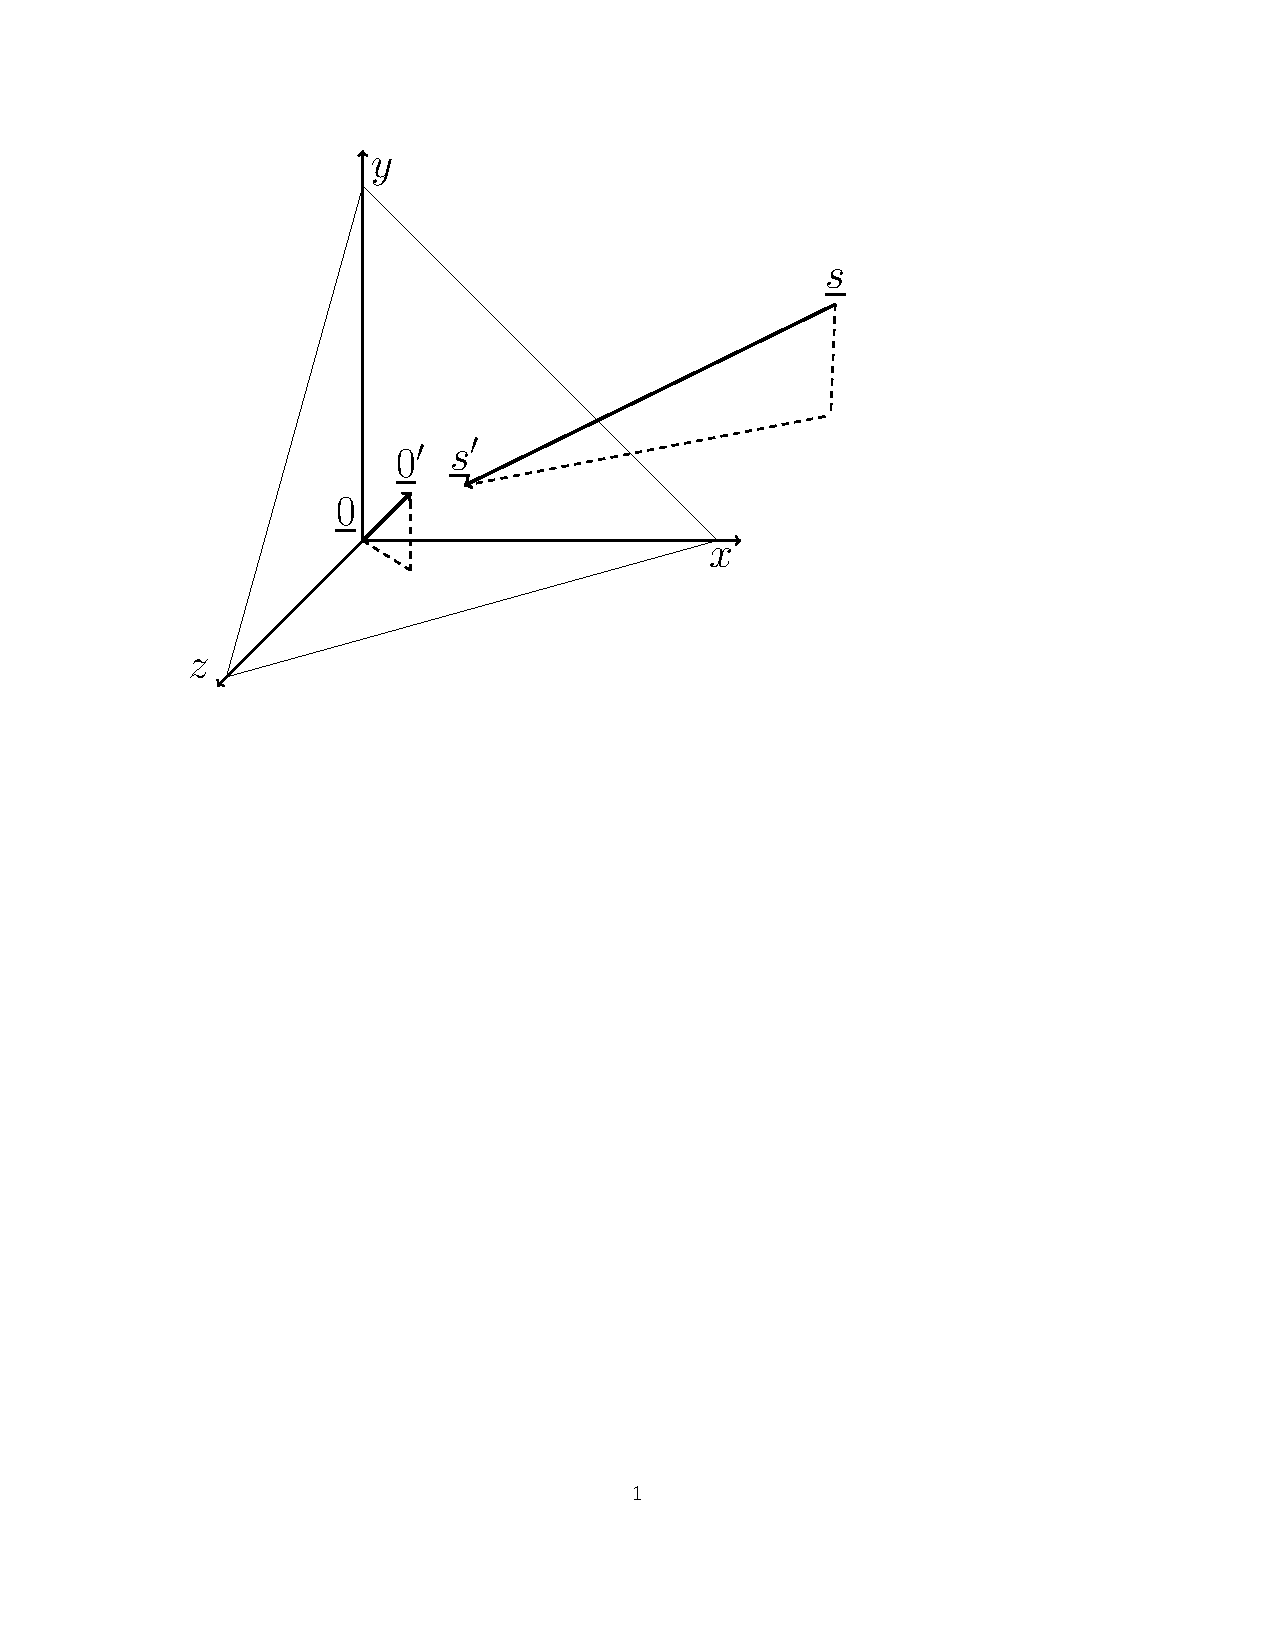
\includegraphics[trim={3cm 16cm 5cm 1cm},clip,scale=0.5]{figures/prob_plot_tikz_bw.pdf}}
%    & \num\putindeepbox[2pt]{\includegraphics[scale=0.25]{figures/real_space_tikz.png}} 
    & \subfigure[]{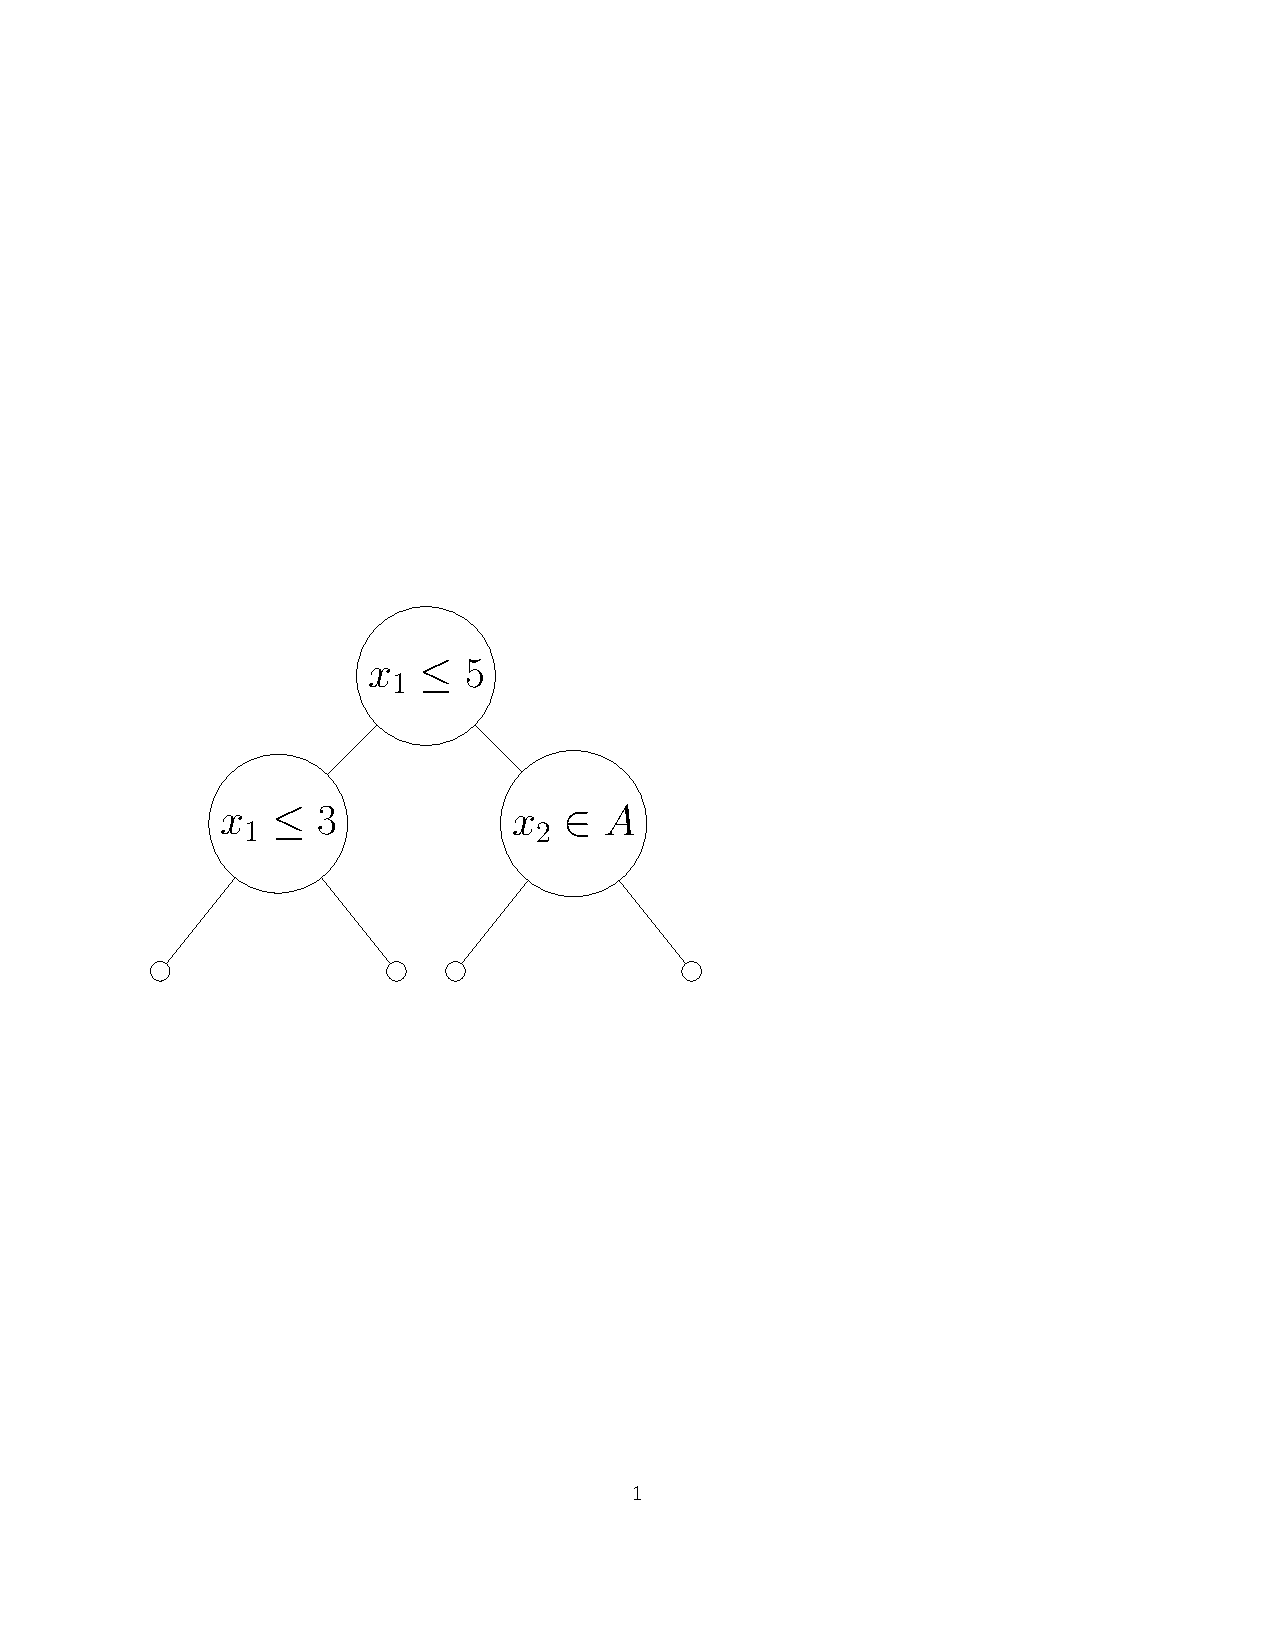
\includegraphics[trim={2cm 11cm 8cm 10.1cm},clip,scale=0.7]{figures/simple_tree_tikz.pdf}} \\
\end{tabular}
  \caption{In (a) we plot the points in the Euclidean space and the primed points represent the points mapped to the probability simplex, represented in the plot by the surface of the triangular plane given by the equation $x+y+z=1, x,y,z >0$. The primes indicate points on the probability simplex after applying the additive logistic transformation to the split counts. In (b) we plot an example decision tree splitting on two of three possible covariates.}
  \label{fig:trees_and_probability}
\end{figure}
 
 Consider Figure \ref{fig:trees_and_probability}; in this figure we have a plot of a decision tree and a plot of the probabilities associated with the tree on a two-dimensional simplex and the three-dimensional Euclidean space. If the observed data has only three covariates and we only observe the first two covariates, $x_1$ and $x_2$ in the estimated tree, then the covariate selection probability vector is approximately $\vec{p} = [0.50, 0.31, 0.19]$. The covariate that has no observed splits receives a lower assigned probability for the subsequent iteration, whereas the two covariates with larger numbers of splits receive proportionally higher covariate selection probabilities for the following iteration of the algorithm. Note the point $\vec{0}^\prime$ in Figure \ref{fig:trees_and_probability} is the point $(1/3,1/3,1/3)$ which functions as the origin on the simplex in 3 dimensions. 

This paper proceeds as follows: Section \ref{sec:Model} contains a description of the models used in this paper. Also in Section \ref{sec:Model}, we state the likelihood function and review the Chipman et al. Bayesian CART \cite{chipman1998bayesian} model for completeness.  In Section \ref{sec:ALoVaS_model}, we present the ALoVaS model, we show the relation with the CGM model, and detail the simulation algorithms used. Then in Section \ref{sec:Examples}, we present simulated examples where we study the efficacy of our proposed method using the regularization priors we describe in Section \ref{sec:Model}. Concluding Section \ref{sec:Examples}, we give an example classifying webpages according to whether those webpages contain ads or not. Finally, in Section \ref{sec:Conclusion} we summarize our findings and discuss the limitations, extensions, and possible variations of our work.      

\section{Bayesian Decision Tree Models}\label{sec:Model}

In Sections \ref{sec:lhood} and \ref{subsec:alt} we describe how we use the ALT to link sparse linear models with covariate selection probabilities facilitating sparse Bayesian decision trees. In Section \ref{subsec:the_tp} we describe the tree prior and the local updates we use to explore the graph of permissible trees. Finally, in Section \ref{subsec:Regularization Priors} we give several examples of regularization priors we will study in our simulated examples.

	\subsection{The Likelihood}\label{sec:lhood}

We begin by reviewing the model proposed in Chipman et al. \cite{chipman1998bayesian}, and show how our approaches generalize upon their model. 

The response data is usually assumed to be observed from a normal or multinomial likelihood function. Nonetheless, other forms of response data such as zero inflated models are possible \cite{Roberts:2014fk}. The likelihood is denoted 

\begin{equation}\label{eqn:cgm_likelihood}
\mathcal{L}(\mathcal{T}, \vec{q}, \vec{\theta} \vert \vec{y} X)=\Pr(\vec{y} \vert X, \mathcal{T}, \vec{q}, \vec{\theta}).
\end{equation} 
		
\noindent Here the $\vec{y}$ denotes the vector of responses, $X$ denotes the matrix of covariates, and $\mathcal{T}$ denotes the tree. The vector $\vec{q}$ is the vector of covariate selection probabilities and $\vec{\theta}$ denotes the vector of parameters in the terminal nodes of the tree. The parameters that we are interested in are: $\mathcal{T}$, $\vec{\theta}$, and $\vec{q}$. We factorize the prior in a similar fashion to Chipman et al. using the breakdown 

\begin{equation}\label{eqn:prior}
\Pr(\mathcal{T}, \vec{q}, \vec{\theta}) \propto \Pr(\vec{\theta} \vert \mathcal{T}) \Pr(\vec{q} \vert \mathcal{T})\Pr(\mathcal{T}).
\end{equation} 

The framework in Chipman et al. \cite{chipman1998bayesian} proposed assumed $\vec{q} \propto 1/p$. Although we find this prior to be a strong \emph{a priori} assumption to take with a large dimensional covariate space, this prior will be seen as a special case of the SSVS prior presented in Section \ref{sec:ALoVaS_model}. Practical difficulties with the uniform prior were already noted in the discussion of Chipman et al. \cite{knight1998bayesian}, although, little work has been done in the interim to remedy this drawback. We modify the framework of Chipman et al. to allow the $\vec{q}$ to vary, depending on their relevance. We specify a prior on the $\mu_j$, a linear space, and use the \ALT\ to determine (indirectly) the prior on the probability space of the $\vec{q}$. This prior specification on the $\mu_j$ allows one to use the methods of the sparse linear model literature but instead apply these methods to decision trees. 

The prior density for $\vec{q}$, the covariate selection probabilities, is defined in Subsection \ref{subsec:alt}. Similar to Chipman et al., we place the uniform prior, denoted $\Pr(\mathcal{T})$, on the decision tree space. We sample the decision trees using the stochastic process defined in Section \ref{subsec:the_tp}.  To monitor the convergence of the Markov chain used to sample the space of decision trees, it is necessary to be able to calculate the marginal density for $\mathcal{T}$ given the covariate selection probabilities $\vec{q}$. This requires choosing conjugate priors for the vector $\vec{\theta}$ so that a closed form marginal density, $\Pr(\vec{y}\vert X,\vec{q},\mathcal{T})$ is available. Thus, if the response data are continuous, we choose a Gaussian density for the prior on $\vec{\theta}$. Similarly, if the response data are categorical, we choose a Dirichlet density as the prior density for $\vec{\theta}$.  

	\subsection{The Additive Logistic Transform}\label{subsec:alt}
	
	The ALT, defined in Equation \ref{eqn:alt}, is a mapping from a Euclidean space to a probability space. 
	%We define our model on a Euclidean space and then, once the draw from the posterior is simulated, we transform the draw to a probability scale using the ALT. 
	The ALT was proposed previously as a fundamental transform for use in compositional data analysis \cite{aitchison1986statistical}. 
	
	The additive logistic normal (ALN) density is obtained as a result of transforming a multivariate normal density using the ALT. The ALN density is given in Equation \ref{eqn:aln}, however we will rarely find use for this equation. Rather, the density on $\vec{\mu}$ is a multivariate normal density with a linear scale. When a probability scale is needed, we apply the ALT to the normal random variates, $\vec{\mu}$, to obtain probabilities. 	
\begin{equation}\label{eqn:aln}
f(\vec{q}\vert \mu, \Sigma) = \left[(2\pi)^p\vert\Sigma\vert\left(\prod_{j=1}^{p}q_j\right)^2\right]^{-1/2}\exp\left[ -\frac{1}{2}(log(\vec{q}_{(p)}/q_{p}) - \vec{\mu})^T \Sigma^{-1}(log(\vec{q}_{(p)}/q_{p}) - \vec{\mu}) \right].
\end{equation} 
In Equation \ref{eqn:aln} the notation $\vec{q}_{(p)}$ indicates a vector with the $p$th entry removed. This density is the result of applying the transformation $q_j = \frac{e^{\mu_j}}{1+\sum_{i=1}^{p-1}e^{\mu_i}}$, for $i=1,\dots,p-1$, and the $p$-dimensional vector, $\vec{\mu}$, has a multivariate normal density with mean vector $\vec{\mu}^\prime$ and covariance matrix $\Sigma$. 
The ALN distribution is defined on the $p-1$ dimensional simplex so that $\sum_{j=1}^{p}q_j =1$. Various settings of the parameters $\vec{\mu}^\prime$ and $\Sigma$ correspond to probabilities concentrated on different regions of the $p-1$ simplex. In practice we do not make use of Equation \ref{eqn:aln}, instead we sample from multivariate normals and transform our random variables using the \ALT. Thus the transformed sampled variates, now representing covariate selection probabilities, have a density defined by Equation \ref{eqn:aln}. To help the reader gain intuition into this distribution, we generate plots for the cases where $\vec{q}$ is a $3$-dimensional vector. The simplex plots illustrate the effect of changes in the multivariate normal parameters on the density in the simplex space. 

In Figure \ref{fig:aln_plots}, the four sub-figures represent sampled observations from a normal distribution after applying the ALT. The extreme points in the simplex correspond to sparse covariate selection probabilities and therefore result in sparse decision trees. In (c), we see data concentrated mostly around the point of the simplex $(1/3,1/3,1/3)$, corresponding to independent standard normals. In sub-figure (d), we see the effect of increasing the variance of the normal densities while maintaining zero means. The larger variances make the draws more likely to come from regions near the edge of the simplex.  In sub-figure (e), we see the effect of adding correlation to the multivariate normal density while keeping the mean vector equal to zero. In this parametrization the density lies close to a plane and after transformation to the simplex space the density is concentrated around a line. In sub-figure (f), we see the result of shifting the mean from the zero to the point $(-2,2,0)$. In our simulation studies the parameter changes will be less pronounced and less isolated. Often we will have the four types of changes presented in these images occurring simultaneously. 

\begin{figure}
\begin{center} 
\begin{tabular}{cc}
  \subfigure[]{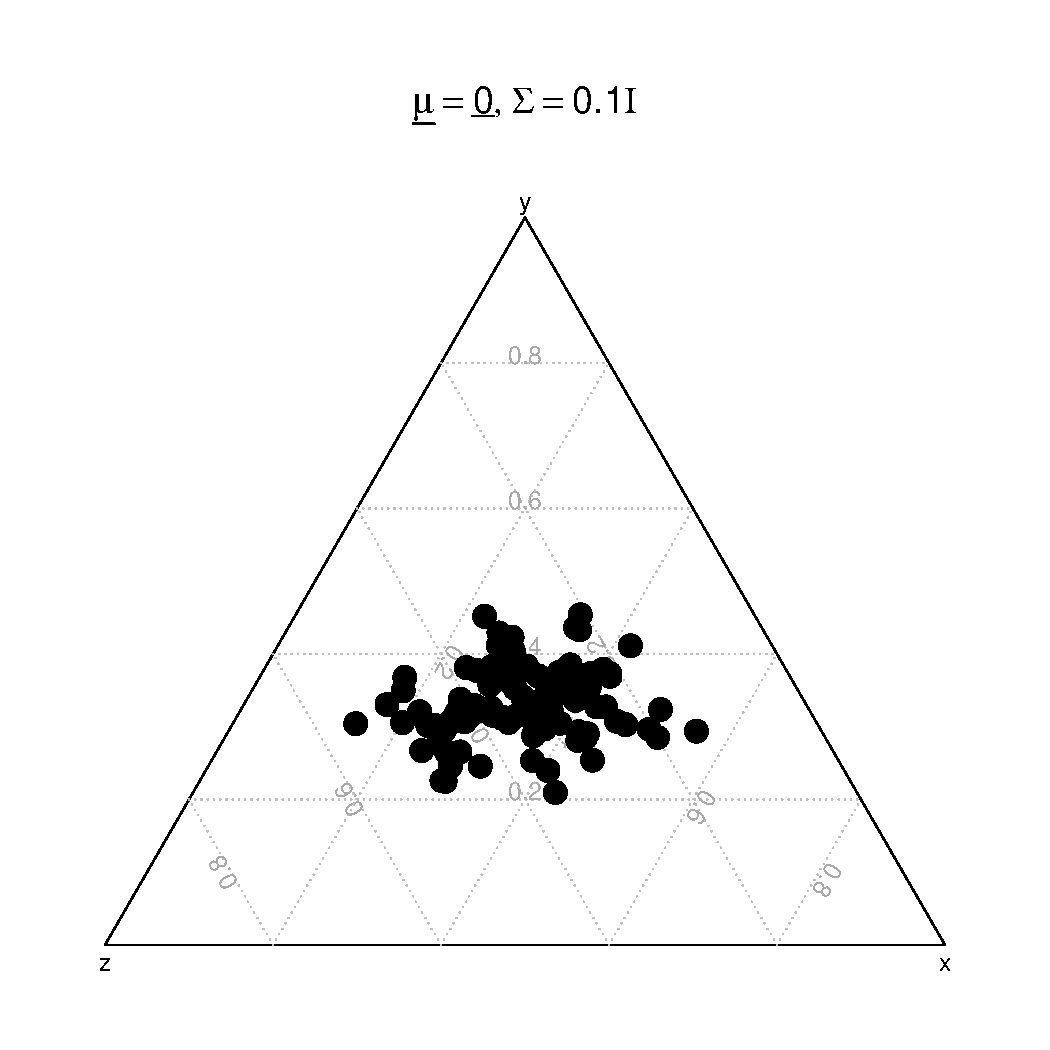
\includegraphics[scale=0.25]{figures/mu0_0_bw.pdf}}
    & \subfigure[]{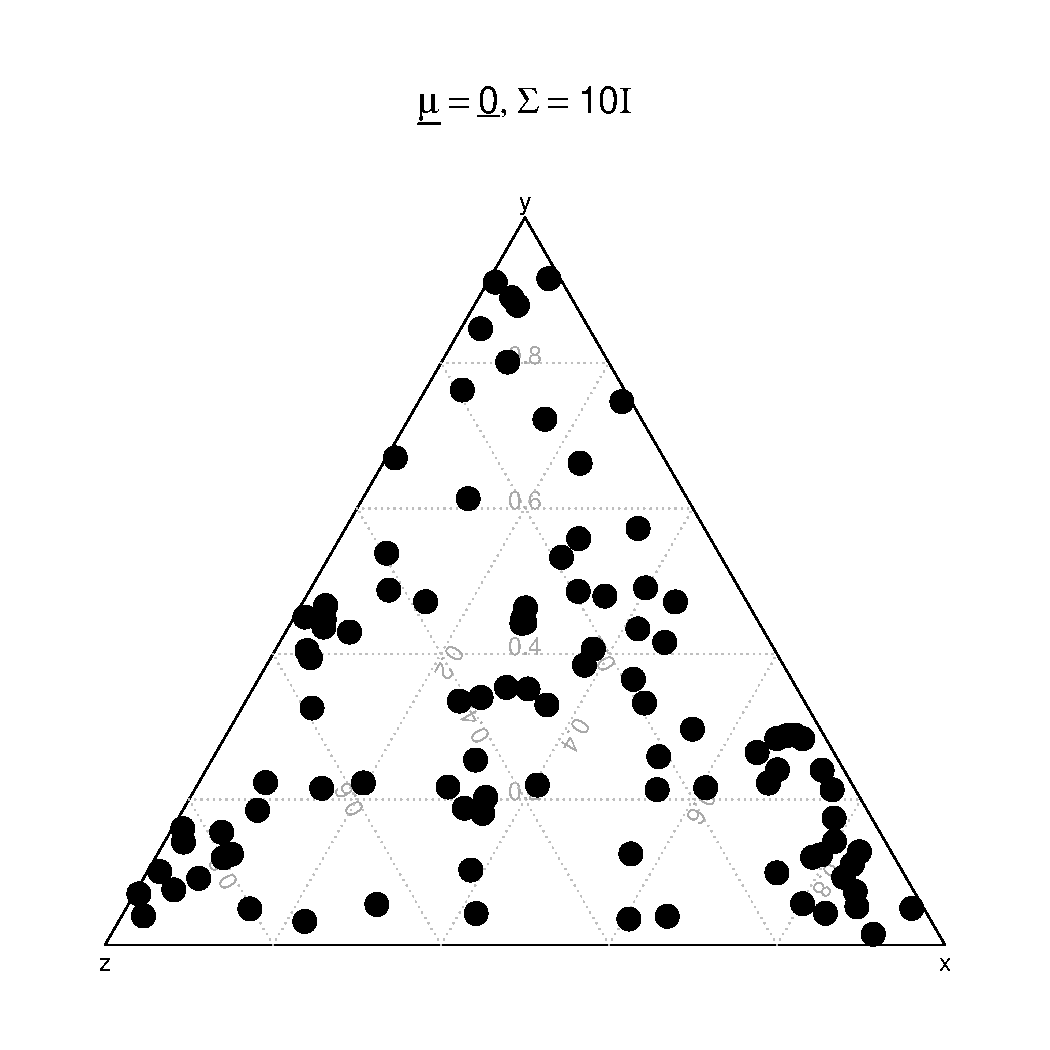
\includegraphics[scale=0.25]{figures/sigma3_3_bw.pdf}} \\
  \subfigure[]{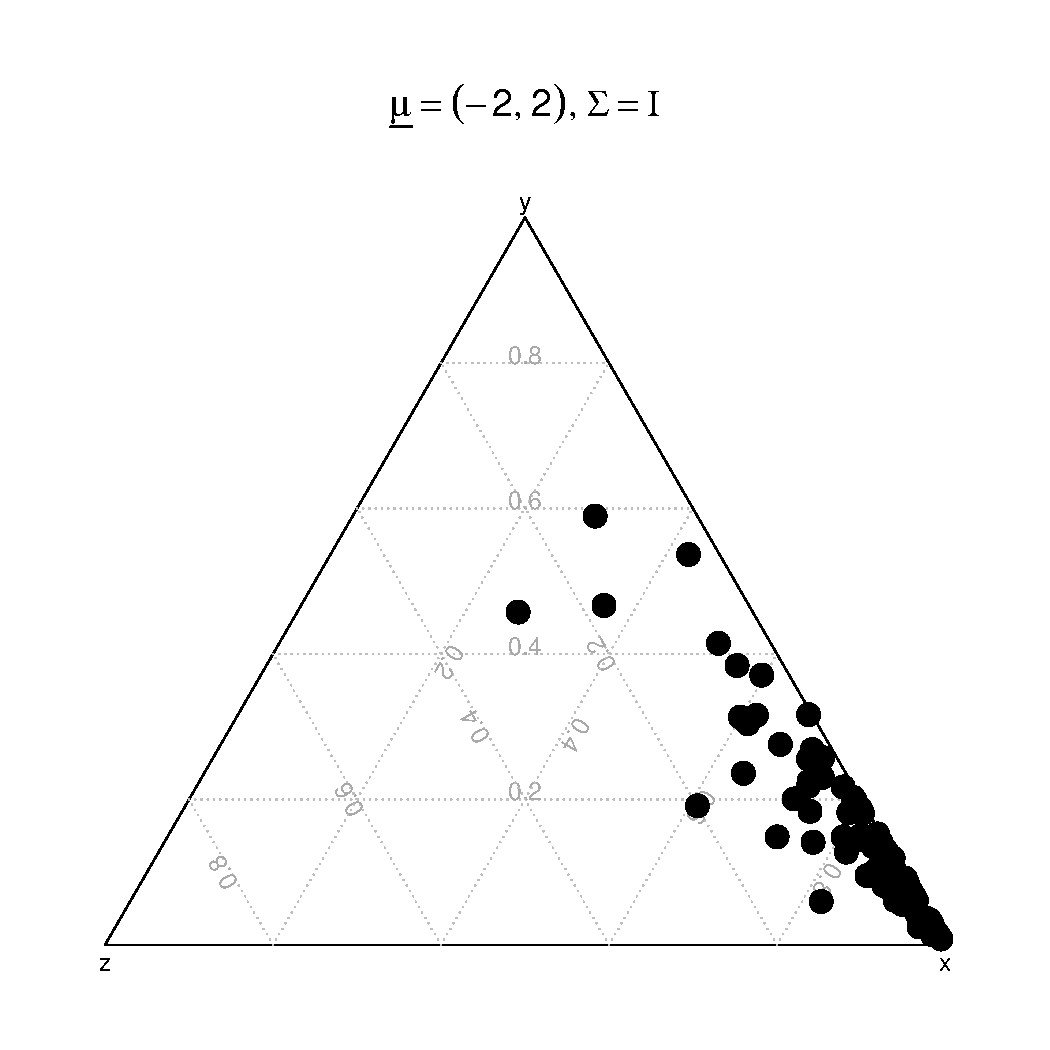
\includegraphics[scale=0.25]{figures/mu2_0_bw.pdf}}
    & \subfigure[]{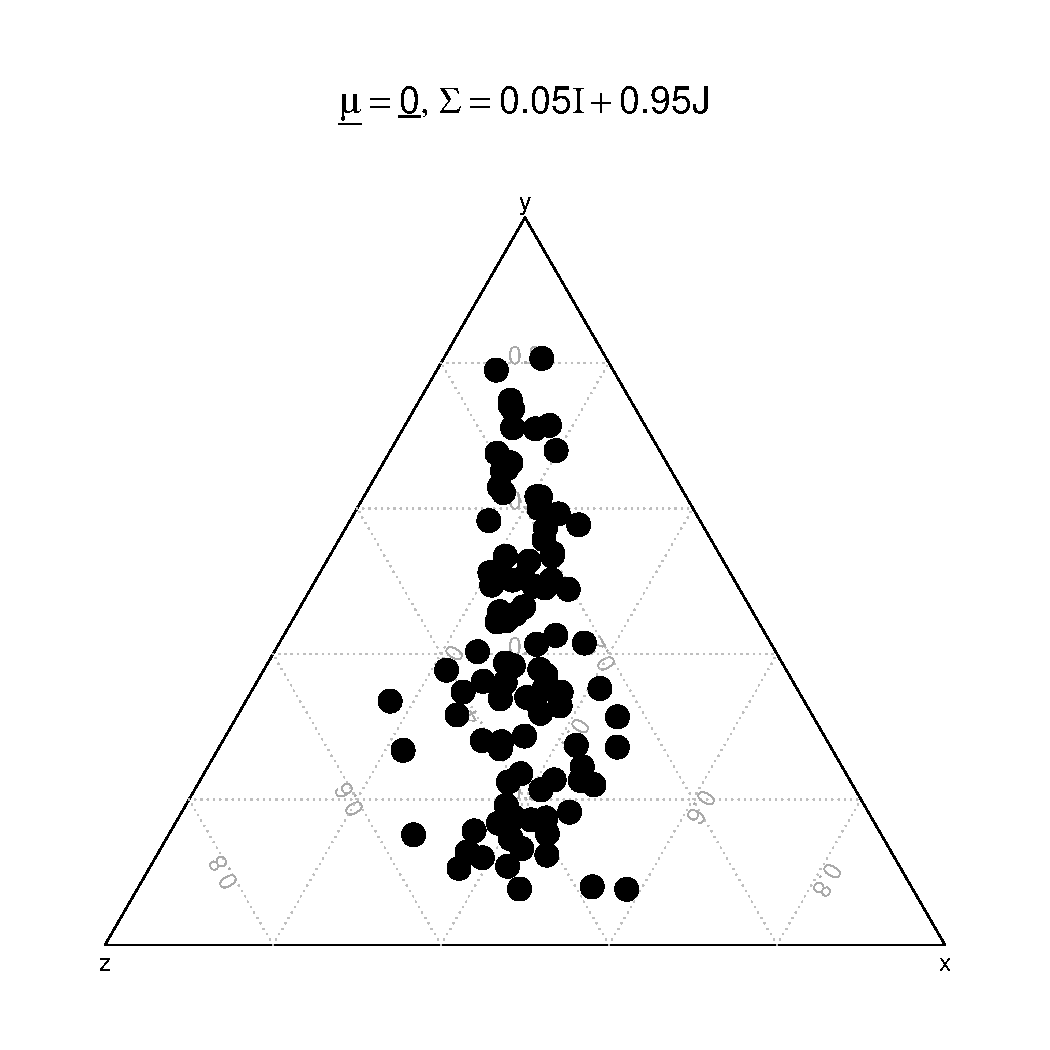
\includegraphics[scale=0.25]{figures/sigma1_9_9_1_bw.pdf}} \\
\end{tabular}
\caption{ALN plots with various multivariate normal parameters. Subfigure (a) contains multivariate standard normal draws. Subfigure (b) plots multivariate normal draws with zero mean and large independent variances. In subfigure (c), contains unit independent variances with mean vector $\mu = (-2,2,0)$. Finally, in subfigure (d) we add correlations while keeping the mean vector as a zero vector. }
\label{fig:aln_plots}
\end{center}
\end{figure}

\subsection{The Tree Prior}\label{subsec:the_tp}	
This section reviews the tree prior first described in Chipman et al. \cite{chipman1998bayesian}, for those readers that are not familiar with the model. Those readers familiar with the paper may safely skip this subsection. 

The tree prior is defined as

\begin{equation} \label{eqn:tree_prior}
\Pr(\mathcal{T}\vert \vec{q}) = \prod_{\eta\in N} \Pr{_{\text{split}}} (\eta) \Pr{_{\text{rule}}}(\eta,j,r_j \vert \vec{q} ),
\end{equation}

\noindent where $\eta$ ranges over all nodes in the tree, denoted by the index set $N$, and the two probabilities in Equation \ref{eqn:tree_prior} are the probabilities of a split at the node $\eta$ and the probability of selecting a specific split rule at node $\eta$ respectively. Also, $r_j$ denotes the splitting value of the split rule at node $\eta$ on the $j$th covariate. The probability of a split in a tree at node $\eta$ is defined by 
 
 \begin{equation}\label{eqn:psplit}
 \Pr{_\text{split}}(\eta)= \alpha(1+d_\eta)^{-\beta},
 \end{equation}
 
\noindent where the quantities $\alpha>0$ and $\beta\geq0$ are fixed values specified \emph{a priori} and $d_\eta = \lfloor lg(\eta)\rfloor$ is the depth of the node $\eta$ ($\lfloor - \rfloor$ denotes the floor function). In this paper $lg$ denotes base 2 logarithms and $log$ denotes base $e$ logarithms. We number the nodes in the tree according to the binary heap node numbering scheme used in many binary tree applications. For a good review of the binary heap node numbering system see Cormen, Lieserson, Rivest, and Stein \cite{cormen2001introduction}. We define the root node, labeled node number one, to have depth zero. Furthermore,  nodes two and three are the left and right child nodes of node one respectively. Both nodes two and three are defined to have depth one. The depths of other nodes in the tree follow similarly.   

  \begin{figure}
  \begin{center}
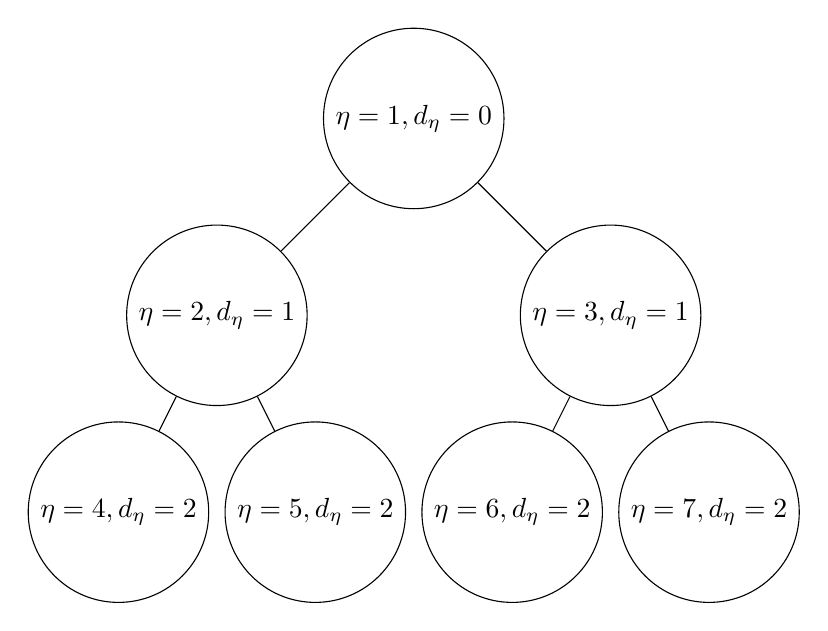
\begin{tikzpicture}
 \node [circle,draw]{$\eta=1,d_{\eta} =0$} [level distance=25mm,sibling distance=50mm]
child { node [circle,draw]{$\eta=2, d_{\eta} =1$} [level distance=25mm ,sibling distance=25mm]
child {node [circle,draw] {$\eta=4, d_{\eta} =2$}}
child {node [circle,draw]{$\eta=5, d_{\eta} =2$}}
}
child {node [circle,draw] {$\eta=3, d_{\eta} =1$} [level distance=25mm ,sibling distance=25mm]
child {node [circle,draw] {$\eta=6, d_{\eta} =2$}}
child {node [circle,draw]{$\eta=7, d_{\eta} =2$}}
};
\end{tikzpicture}

\caption{The binary heap node numbering system used in our simulations. }
\label{fig:tree_node_nums}  
\end{center}
\end{figure}
In addition to the process prior defined on the tree, we define a process prior on the selection of covariates for split rules within a tree. The function $\Pr{_{\text{rule}}}(\eta,j,r_j \vert \vec{q} )$ is decomposed into two components, one selecting the $j$th covariate which we use to propose a split at the node, and a second component selecting a specific split value ($r_j$). This corresponds to the conditional probability decomposition 

\begin{equation}\label{eqn:decomp}
\Pr{_\text{rule}}(\eta,j,r_j\vert \vec{q}) = \underbrace{\Pr{_\text{cov}}(j,\eta \vert \vec{q})}_{\text{ALN density}} \underbrace{\Pr{_\text{split value}}(r_j \vert j, \eta)}_{\text{Uniform}}.
\end{equation}

\noindent The tree prior, denoted $\Pr(\mathcal{T})$, is defined uniformly over the space of admissible trees. Exact enumeration of all admissible trees is only possible for very small values of $n$, the number of observations. The number of admissible trees is a cumulative sum of Catalan numbers less than or equal to a given depth. This sum grows at the rate $\mathcal{O}(4^n/n^{3/2})$ \cite{mattarei2009asymptotics}, the same rate as the Catalan numbers themselves, displayed in Figure \ref{fig:asymptotics}, and becomes intractable quickly. Fortunately, Markov chain Monte Carlo sampling allows us to sample from the space of trees using a Metropolis-Hastings rule with local proposals on the space of trees. We now detail the structure of the proposal functions. 

\begin{figure}[H]
  \centering
  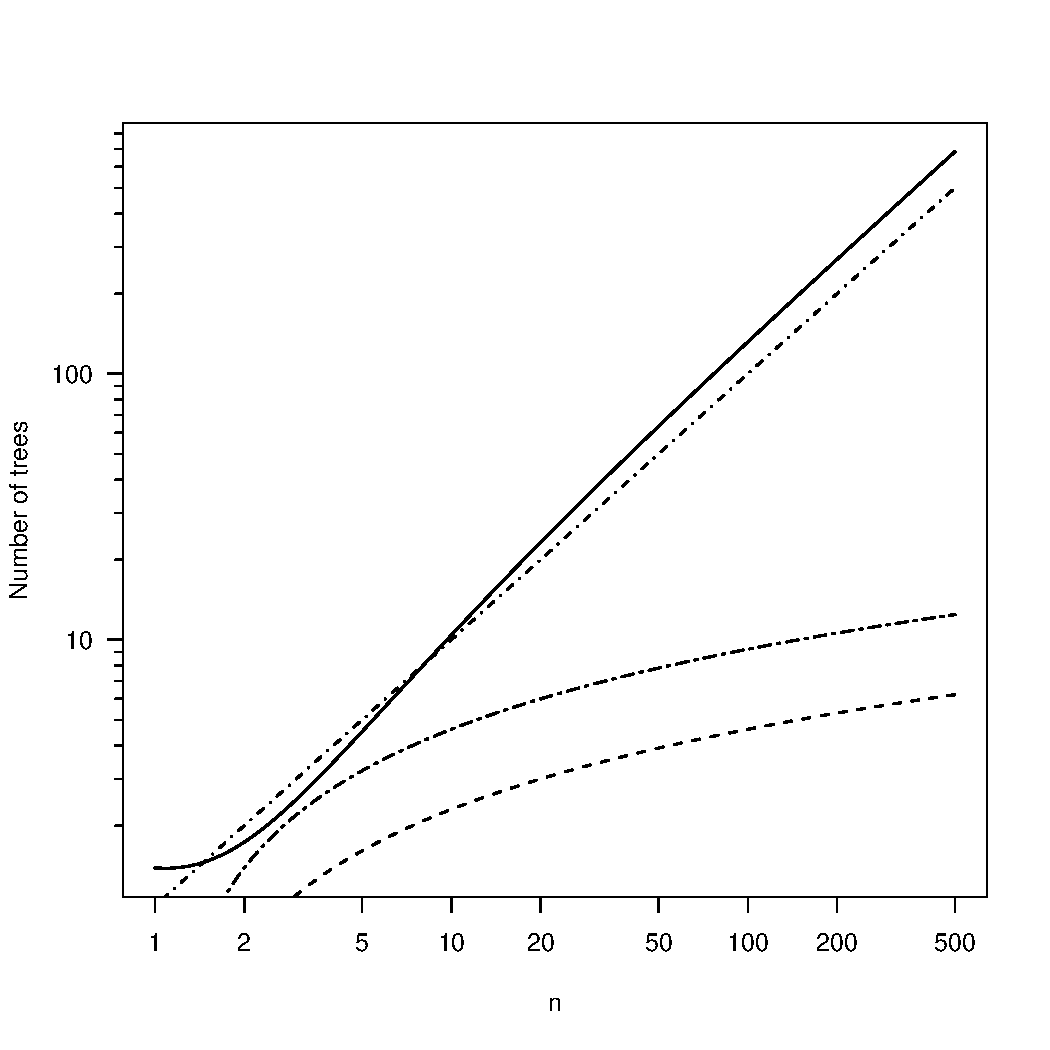
\includegraphics[width=4in]{figures/asymptotics_plot_bw.pdf}
  \caption{Plots of the log of the number of possible trees (solid line) less than or equal to a given depth $n$, compared to exponential (45 degree line), quadratic (dash-dotted line) and linear functions (even-dashed line). Note the vertical axis is on a log scale.  }
  \label{fig:asymptotics}
\end{figure}

Given a tree $\mathcal{T}$, we sample a new tree adjacent to $\mathcal{T}$ by proposing local updates. The local updates we use are the following: 

\begin{itemize}
 \item The Grow step: choose at random one of the terminal nodes and propose to append two new child nodes with probabilities given by Equation \ref{eqn:psplit}. 
 \item The Prune step: the reverse of the grow step, a terminal node is selected at random and the selected node and that selected node's sibling are both pruned to the immediate parent of the two child nodes. The parent node becomes a terminal node. 
 \item The Change step: randomly pick an internal node and propose to change the split rule at the selected node with that of another observation, possibly on a different covariate.
  \item The Swap step: randomly select an internal node that is not the immediate parent of any terminal node and proposes to swap the split rules of the parent-child pair. Otherwise, when both child nodes split on the same covariate, both child node's rules and the parent node's rules are swapped.
  \item The Rotate step: randomly choose a left or right rotation move, each with probability $1/2$. Then a rotatable node is chosen and a rotate move is performed.
 \end{itemize}
  The rotate operation for binary trees was first introduced in Sleator and Tarjan \cite{sleator1985self} and was implemented with Bayesian decision trees by Gramacy and Lee \cite{gramacy2008bayesian}. The rotate move was originally suggested by Knight, Kustra, and Tibshirani \cite{knight1998bayesian} as another possible move that might improve mixing. A good introduction and several practical uses of the rotate move can be found in Cormen, Lieserson, Rivest, and Stein \cite{cormen2001introduction}. The proposal functions in Gramacy and Lee \cite{gramacy2008bayesian} perform a rotate move only when a swap move is proposed and the parent-child pair both split on the same covariate. We modify this and allow rotate moves to be a separate proposal function and not a special swap move case. The proposal mechanism of Chipman et al. uses the grow, prune, change and swap moves only. In addition, neither Chipman et al. \cite{chipman1998bayesian}, Denison et al. \cite{denison1998bayesian}, nor Gramacy and Lee \cite{gramacy2008bayesian} included weights on each covariate in their examples or model specifications. They sampled each covariate and each split value uniformly across all covariates. 

	\subsection{Regularization Posteriors}\label{subsec:Regularization Priors}
		While this paper is focused on regularized trees, we will show the connection to various regularization frameworks used for regression models. In essence, the ALoVaS method can incorporate any model based regularization method. We briefly describe a few popular approaches for the sake of completeness. 
		
		Regularization, originally defined as a constrained optimization problem, has been a popular topic of research in the sparse linear model literature. The lasso model \cite{tibshirani1996regression}, a popular regularization technique, seeks to optimize an $L_1$ constrained least squares problem. The negative of the log posterior density of the lasso is given by Equation \ref{eqn:lasso_obj}
		
		\begin{equation}\label{eqn:lasso_obj}
		-log(\pi(\vec{\mu} \vert \vec{y}, X, \lambda )) \propto \sum_{i=1}^n\left(y_i - \vec{x}_i^T\vec{\mu}\right)^2 + \underbrace{\lambda \sum_{j=1}^p \vert \mu_j \vert}_{\text{$-log$ Laplace prior}}\hspace{-0.5cm}.
		\end{equation}
		
\noindent Interpreted in a Bayesian setting, the $L_1$ constraint is viewed as a double exponential or Laplace prior on the coefficients, $\mu_j$. A nice property of the lasso model is that the \emph{maximum a posteriori} estimated coefficients form a sparse vector, with $\lambda$ controlling the degree of sparsity. Thus, one of the models that we will use in our simulations uses a lasso prior to constrain the covariate selection probabilities. 

Since the publication of the lasso model, several other regularization techniques have been published. One that predates the lasso by several years is the Stochastic Search Variable Selection method (SSVS) \cite{george1993variable}, given in Equation \ref{eqn:ssvs} beneath
	\begin{equation}\label{eqn:lasso_obj}
		-log(\pi(\vec{\mu} \vert \vec{y}, X, \pi, \sigma, \psi )) \propto \sum_{i=1}^n\left(y_i - \vec{x}_i^T\vec{\mu}\right)^2 + \sum_{j=1}^p log\left\{\underbrace{ \pi_jN(0, \sigma^2)+(1-\pi_j)N(0, \sigma^2+ \psi^2)}_{\text{Spike \& slab prior}}  \right\},
		\end{equation}
with $\sigma < \psi$ and where $N(A,B)$ denotes the likelihood of a normal random variate with mean $A$ and variance $B$. This Bayesian method posits a prior distribution that is a point mass mixture prior. The point mass is at zero and the density is a normal distribution, with a Bernoulli random variable mixing the two. %Although this method is often useful in practice, recently some theoretical arguments have called the use of normal densities in to question when compared to other priors studied by Johnson and Rossell \cite{johnson2010use} called moment priors. Moment priors are defined in the Appendix in Equation \ref{eqn:moment_prior}.  We do not advocate the use of either the moment or SSVS prior over the other. However, 
We present simulation studies that use the SSVS model. In addition to these two methods, SSVS and lasso, we also study another prior known as the horseshoe prior, originally proposed by Carvalho, Polson, and Scott \cite{carvalho2010horseshoe} and further studied in Polson and Scott \cite{polson2010shrink}. This prior may also be viewed as a constraint on the unknown coefficients, although the objective function is usually viewed in a Bayesian context as a posterior distribution over the coefficients. The horseshoe model has the following negative log posterior, 
\begin{equation}\label{eqn:horseshoe}
		-log(\pi(\vec{\mu} \vert \vec{y}, X, \sigma, \lambda )) \propto \sum_{i=1}^n\left(y_i - \vec{x}_i^T\vec{\mu}\right)^2 + \underbrace{\sum_{j=1}^p\left(\frac{\mu_j}{\lambda_j\sigma} \right)^2 + \frac{p+1}{2}log\left(1+ \frac{\lambda_j^2}{p}\right)}_{ \text{$-log$ Horseshoe prior} }.\end{equation}
\noindent Although Carvalho et al.  \cite{carvalho2010horseshoe} state that the horseshoe prior is the case when $\sigma^2=1$, in their paper they refer to the general case of $\sigma^2$ as the horseshoe prior and we also call the general case the horseshoe prior. Also, $\lambda^2$ has a central half-t density with $p$ degrees of freedom. Here for completeness, we write out the the priors, including the hierarchical form of the horseshoe prior which is the commonly used way to represent the horseshoe prior:
\begin{equation}\label{eqn:ssvs}
\pi(\mu_j) \propto N(0,\sigma_j^2)p_j+(1-p_j)N(0,\sigma_j^2+\psi),
\end{equation}
\begin{equation}\label{eqn:lasso}
\pi(\mu_j) \propto \exp(-\lambda\vert \mu_j\vert),
\end{equation}
\begin{align}\label{eqn:horseshoe}
\pi(\mu_j\vert \lambda_j) &\propto N(0, \lambda^2\sigma^2),\\
\pi(\lambda_j | a)&\propto \text{Inv-}\Gamma(a,b),\nonumber \\ \nonumber
\pi(a)&\propto \text{Inv-}\Gamma(c,d).
\end{align}
The reader should note that the Laplace prior in the model indicates that this is a lasso type model and the lasso prior is in fact a double exponential, or Laplace prior. Other priors on the $\mu_j$ are possible and we consider the SSVS, or spike and slab prior given in Equation \ref{eqn:ssvs}, and the horseshoe prior given in Equation \ref{eqn:horseshoe}, in addition to the lasso prior of Equation \ref{eqn:lasso}. 

Recall, if $X$ is distributed according to a t-distribution with $p$ degrees of freedom, then $Y=\vert X\vert$ is distributed according to a half-t distribution with $p$ degrees of freedom \cite{johnson1995continuous}. For our simulations, we use the mixture representation of the half-t distribution given in Huang and Wand \cite{huang2013simple} and given in Appendix \ref{sec:appendix} for completeness. Interestingly, the three models can be interpreted as scale mixtures of normal priors. The Lasso is equivalent to a exponential scale mixture of normals, the SSVS is a point mass scale mixture of normals, and the horseshoe is a half-t scale mixture of normals. In all three cases we have a global regularization parameter, $\lambda$, $\psi$, and $\sigma$ represent the regularization parameters for the lasso, SSVS and horseshoe priors respectively.    

\section{The ALoVaS Model}\label{sec:ALoVaS_model}

In this section we detail the ALoVaS model in the most general form. Then we detail the model for an arbitrary choice of priors for the means and variances. This allows the reader to see concrete examples of the ALoVaS method for clarity while preserving the general applicability of the method. 

We begin the model description by stating our posterior, 
\begin{equation}\label{eqn:post}
\pi(\mathcal{T}, \theta, \vec{q} \vert Y,X) \propto \mathcal{L}(Y \vert X, \mathcal{T}, \theta, \vec{q})\pi(\theta \vert \mathcal{T})\pi(\vec{q}\vert \mathcal{T})\pi(\mathcal{T}), 
\end{equation}
where $Y$ denotes the response vector, $X$ is the design matrix or the collection of covariates, $\mathcal{T}$ denotes the decision tree, and $\vec{q}$ denotes the vector of covariate selection probabilities. 

Instead of defining $\pi(\vec{q} \vert \mathcal{T})$ in terms of $\vec{q}$ we define on a linear scale, and once we have the linear scale parameters we convert to a probability using the \ALT
\begin{equation}\label{eqn:alt}
\vec{q} = \left[ q_1, q_2,\dots, q_{p-1}, q_p \right] =\vec{g}^{-1}(\vec{\mu})= \left[ \frac{e^{\mu_1}}{1+S_{p-1}},\frac{e^{\mu_2}}{1+S_{p-1}}, \dots,\frac{e^{\mu_{p-1}}}{1+S_{p-1}},\frac{1}{1+S_{p-1}} \right],
\end{equation} 
where the notation is the same as in Section \ref{sec:Introduction}. The parameters on the linear scale are denoted $\mu_j$ and can be interpreted as log-odds of selecting covariate $j$. The number of splits on each covariate at each iteration are denoted as $s_{jt}$. We assume these to have an approximately normal distribution once multiplied by a parameter $c_j$. The parameter $c_j$ is distributed on the support $[-1,1]$ and has a scaled-beta prior scaled and shifted to cover the support of $c_j$. This framework is written succinctly in Equations \ref{eqn:alovas1} and \ref{eqn:alovas2}. These equations are written out here for completeness

\begin{equation}\label{eqn:alovas1}
c_js_{jt} \vert c_j \sim N\left(\mu_j=log(q_j/q_p),\sigma_j^2\right),
\end{equation}

\begin{equation}\label{eqn:alovas2}
c_j \sim \text{ ScaledBeta}(-1,1,\alpha, \beta), \text{   and}	
\end{equation}

\begin{equation}\label{eqn:flavor_prior}
\mu_j \sim g(\mu_j). 
\end{equation}

Here the density function $g$ can be specified by the analyst. In this paper we detail the specification of $g$ as a double exponential (Equation \ref{eqn:lasso}) prior, SSVS (Equation \ref{eqn:ssvs}) prior, and horseshoe (Equation \ref{eqn:horseshoe}) prior. The form of $g$ should now be recognized as a regularization prior. In Appendix \ref{sec:appendix} we include details for each of the three stated priors. Namely, the pseudocode for the lasso, SSVS, and horseshoe priors may be found in Sections \ref{sec:lasso_app}, \ref{sec:ssvs_app}, and \ref{sec:horseshoe_app}, respectively.
Finally, we assume the usual Jeffreys' prior for the variances, 
\begin{equation}
\pi(\sigma^2_j) \propto \ \  \sigma^{-2}_j. 
\end{equation}

In practice inference should not be conducted on all the parameters in the model. There are many additional parameters in this model compared to the CGM version. For us, the main parameters of interest are $\mathcal{T}_i$, the $i$th decision tree and $\vec{q}$, the covariate selection probabilities. The probabilities are a function of the parameters $\vec{\mu},\vec{c},\vec{\sigma}$ and any other hyper-parameters estimated or sampled over. For full implementation details of the ALoVaS methods we study we include pseudocode in Appendix \ref{sec:appendix} for the SSVS, lasso, and horseshoe methods we implement. However, as noted in this section, different choices of $g(\mu_j)$ priors that regularize will result in different types of ALoVaS methods so the careful reader should be able to tailor the existing methods to whatever specific regularization prior they desire. 

 %We now describe the detailed balance criteria and give the equation that must be satisfied for this criteria to hold in our model. 
 The proposed trees are accepted or rejected based on the usual Metropolis-Hastings rule which is written here for completeness
 
 \begin{equation}
\alpha(\mathcal{T}\vert \mathcal{T}^\prime) = \text{min}\left(\frac{\Pr(\mathcal{T}^\prime \vert X, \vec{q}, \vec{y} )\Pr(\mathcal{T}| \mathcal{T}^\prime) }{ \Pr(\mathcal{T} \vert X, \vec{q}, \vec{y})\Pr(\mathcal{T}^\prime \vert \mathcal{T}) } ,1\right)
 \end{equation}
 
Detailed balance is a formal property imposed on Markov Chains after convergence. Intuitively, the detailed balance equation indicates that after convergence the process has the same distribution when run forwards in time as when run backwards in time. Formally, this is represented in Equation \ref{eqn:detailed_balance}, 
\begin{equation}\label{eqn:detailed_balance}
\alpha (\mathcal{T}^{(t)} \vert \mathcal{T}^{(t-1)}, \vec{q}^{(t-1)})\pi(\mathcal{T}^{(t)}\vert \vec{q}^{(t-1)})\pi(\vec{q}^{(t-1)}) = \pi(\vec{q}^{(t)}\vert \mathcal{T}^{(t-1)})\pi(\mathcal{T}^{(t-1)})\alpha(\mathcal{T}^{(t-1)} \vert \mathcal{T}^{(t-1)}, \vec{q}^{(t)} ),
\end{equation}
where the superscripts denote the (discrete time) nature of the Markov Chain. Where we are holding the $\vec{q}$ constant while transitioning from $\mathcal{T}^{(t)}$ to $\mathcal{T}^{(t-1)}$. Once the transition on $\mathcal{T}$ has been made we update $\vec{q}$ using a Gibbs step. Thus, our algorithm is a Metropolics within Gibbs algorithm. The Metropolis step updates $\mathcal{T}$ and the Gibbs step updates $\vec{q}$ and we iterate until convergence. It can be shown that any algorithm satisfying the detailed balance criteria is guaranteed to converge to the stationary distribution \cite{robert1999monte}. 

The Markov Transition Density (MTD),  for $q_j$ is given by Equation \ref{eqn:markov_trans_density}
\begin{equation}\label{eqn:markov_trans_density}
\Pr(q_j^{(t)}\vert q_j^{(t-1)})=\sum_{\mathcal{T}}\Pr(q_j^{(t)}\vert \mathcal{T}^{(t-1)})\Pr(\mathcal{T}^{(t-1)} \vert q_j^{(t-1)}).
\end{equation}
A similar MTD can be formulated for $\mathcal{T}$. When closed forms exist for these MTDs, and minorization and drift conditions are also satisfied, geometric convergence may be established. For examples and more details on this line of study, see the very readable introduction by Jones and Hobert \cite{jones2001honest}. For our example, the MTD for $\vec{q}$ involves evaluating an NP-Hard sum, thus exact convergence rates seem unlikely to be found. 

In this section we write out the ALoVaS model for a specific regularization prior. In general, the prior on the set $\{\mu_j,\sigma^2_j\}_{j=1}^{p}$ will change, giving us different flavors of the ALoVaS method. In this paper we include a study of the lasso, horseshoe, and SSVS priors, but other variations are certainly possible. Moreover, we do not claim optimality of our results. Indeed, many of these priors are optimal only in specific circumstances. If a model is not optimal in a linear model, this will carry over to our ALoVaS model and therefore, the ALoVaS method will be sub-optimal as well. This is not a drawback of our proposed ALoVaS method but is a drawback of the choice of the regularization prior in the given situation.  
